\chapter{Redukcja argumentów}
\label{chapter:reduction}

Algorytm generowania indeksów zaproponowany przez profesora Sasao pozwala na zastosowanie pamięci o~mniejszym rozmiarze niż wskazywałaby na to liczba argumentów.
Nie jest to oczywiście jedyna metoda pozwalająca na uzyskanie takiego efektu.
W~niniejszej pracy przedstawione zostało podejście wykorzystujące jednocześnie redukcję i~kompresję argumentów.

Redukcja argumentów jest to proces pozwalający na zmniejszenie liczby parametrów wejściowych funkcji,
poprzez odrzucenie argumentów zawierających wyłącznie redundantne dane.
Po wykonaniu takiego procesu,
próba usunięcie kolejnego argumentu z~funkcji wyjściowej powoduje kolizję wierszy o~różnych wartościach i~tym samym utratę informacji.
Zbiór argumentów powstały w~wyniku redukcji nazywamy reduktem i oznaczamy $R$.
Istnieje wiele sposobów redukcji argumentów.
Należą do nich metody systematyczne
pozwalające na znalezienie wszystkich minimalnych rozwiązań,
jak i~heurystyczne,
charakteryzujące się szybszym działaniem.
Sama redukcja nie zawsze przynosi spektakularne rezultaty.
Dla skrajnych przypadków funkcji $F$,
w~których każdy argument dostarcza niezbędnej informacji,
redukcja może nie przynieść żadnego efektu.
Niezbędna wtedy jest,
opisana w~dalszej części pracy,
kompresja argumentów.

\section{Problem złożoności}

Do problemu redukcji argumentów można podejść w~sposób intuicyjny.
Można próbować po kolei usuwać argumenty i~weryfikować spójność danych.
W~przypadku utraty spójności usuwany argument musiałby się znaleźć w~końcowym rozwiązaniu.
W~przeciwnym przypadku należałoby go usunąć i~kolejne weryfikacje przeprowadzać z~jego wyłączeniem.
Pojedyncza weryfikacja wymaga porównania każdych dwóch wierszy o~różnej wartości funkcji.
Jeżeli funkcja ma $n$~argumentów oraz $m$ wierszy wtedy porównanie dwóch dowolnych wierszy odbywa się ze złożonością liniową $O(n)$.
Liczba par wierszy do porównania wynosi,
w~zależności od rozkładu wartości funkcji,
od $m$ do $m^2$.
Zatem złożoność obliczeniowa pojedynczej weryfikacji to $O(n \cdot m^2)$.
Taką weryfikację trzeba przeprowadzić dla każdego z~$n$~argumentów co daje końcową złożoność $O(n^2 \cdot m^2)$.

Problem takiego podejścia,
poza złożonością,
leży dodatkowo w~jakości uzyskiwanego rozwiązania.
W~procesie redukcji argumentów część z~nich może być ważniejsza
i~tym samym pozostawienie takiego argumentu może pozwolić na usunięcie dwóch (lub nawet więcej) innych.
Oznacza to,
że wynik takiej redukcji,
mimo iż jest prawidłowy,
często nie jest optymalny.

\section{Minimalne pokrycie kolumnowe}

Innym sposobem wyboru argumentów w~czasie redukcji jest dobieranie argumentów,
aż do zapewnienia pełnej rozróżnialności.
Zaczynamy z~jednym argumentem i~kolejno wybieramy kolejne,
które znajdą się w~końcowym rozwiązaniu.
Jeżeli przy takim podejściu dodatkowo będziemy w~stanie ocenić,
które argumenty są bardziej wartościowe to uzyskamy lepsze wyniki.

Za wagę argumentu w~redukcie można przyjąć liczbę rozróżnień,
których on dostarcza.
Jeżeli dzięki jednemu argumentowi jesteśmy w~stanie rozróżnić tylko jedną parę wierszy o~różnych wartościach,
to ma on mniejszą wagę od takiego,
który rozróżnia kilka par wierszy.
Z drugiej strony nawet argument,
który dostarcza jednego rozróżnienia,
będzie istotny,
jeżeli żaden inny argument nie dostarcza takiego rozróżnienia.

Informacje o~tych zależnościach uzyskuje się z~macierz rozróżnialności (oznaczana $MR$), nazywanej również tablicą porównań,
która zawiera wynik operacji XOR wszystkich par wierszy o~różnych wartościach funkcji.
Przykładowo na rysunku \ref{fig:discernibility-table} pierwszy wiersz macierzy powstaje z porównania wierszy 1 i 3.
Wiersze 1 z 2 oraz 3 z 4 nie są porównywane ze względu na taką samą wartość funkcji.
Jedynki w~takiej macierzy obrazują,
które argumenty dostarczają rozróżnień między zadanymi parami wierszy.
Na potrzeby niniejszej pracy macierz rozróżnialności nie jest pozbawiana wierszy pokrywanych przez inne zgodnie z~rachunkiem kostek boolowskich.
Takie wiersze nie są istotne z~punktu widzenia znajdowania minimalnego pokrycie kolumnowego,
ponieważ istnieją inne wiersze, których obecność w macierzy zapewnia dostarczenie wystrczających rozróżnień.
Mimo to szybszym rozwiązaniem jest pozostawienie ich w macierzy,
gdyż ich usunięcie wymaga porównania wszystkich wierszy każdy z~każdym
i~jest nie opłacalne ze względu na złożoność obliczeniową.
Z~drugiej strony w~przypadku dekompozycji liniowej wiersze te są niezbędne do prawidłowego przeprowadzenia algorytmu i~nie mogą być usunięte.
Zarówno algorytm usuwania jak i~jego złożoność zostały dokładnie wyjaśnione w~pracy dyplomowej \cite{inzynierka}.

\begin{figure}[h]
\centering
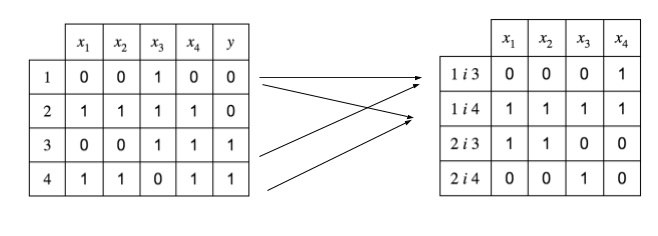
\includegraphics[width = 13cm]{chapter02/discernibility-table.png}
\caption{Proces powstawania tablicy rozróżnialności (źródło własne).}
\label{fig:discernibility-table}
\end{figure}

Znalezienie reduktu,
przy użyciu tablicy rozróżnialności sprowadza się do problemu znalezienia minimalnego pokrycia kolumnowego,
czyli takiego zbioru kolumn,
dla którego w~każdym z~wierszy znajduje się co najmniej jedna jedynka.
Najprostszy algorytm znajdujący takie rozwiązanie sprowadzałby się do następujących kroków:
\begin{enumerate}
\item Wybranie kolumny o~największej liczbie jedynek,
\item Usunięcie wierszy z~jedynkami w~tej kolumnie,
\item Powtarzanie do uzyskania pustej macierzy.
\end{enumerate}

Nie uwzględnia on jednak faktu,
że niektóre rozróżnienia są dostarczane przez mniejszą liczbę argumentów niż inne.
Najłatwiej zauważyć to na przykładzie argumentów niezbędnych, znajdującym się na rysunku \ref{fig:required-arguments}.
W~ich przypadku istnieją takie wiersze,
które zawierają wyłącznie po jednej jedynce (wiersze 1 i 2).
Oznacza to,
że argument odpowiadający tej jedynce jest niezbędny do uzyskania minimalnego pokrycia kolumnowego.
Taki argument często dostarcza innych rozróżnień,
które przy użyciu proponowanego powyżej algorytmu zawyżałyby sztucznie wagę innych argumentów.
W przypadku fukncju z rysunku \ref{fig:required-arguments},
argument $x_2$ posiada najwięcej jedynek i~jednocześnie jest nadmiarowy,
gdyż w minimalnym rozwiązaniu i tak muszą znaleźć się argumenty niezbędne $x_1$ i $x_3$.

\begin{figure}[H]
\centering
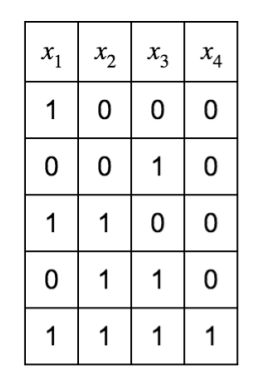
\includegraphics[width = 5cm]{chapter02/required-arguments.png}
\caption{Przykład obrazujący niedoskonałości algorytmu największej liczby jedynek (źródło własne).}
\label{fig:required-arguments}
\end{figure}

Aby uwzględnić problem sztucznego zawyżania wag argumentów,
w~ostatecznym rozwiązaniu sposób wyboru kolumny jest dwuetapowy.
Najpierw znajdowany jest wiersz o~najmniejszej liczbie jedynek ($w_j$),
następnie wybierana jest kolumna ($x_i$),
która ma najwięcej jedynek oraz jedynkę w~wybranym wierszu ($x_{i_{w_j}} = 1$).
Takie rozwiązanie wyboru kolumn często prowadzi do uzyskania reduktu o~najmniejszej liczności \cite{unate-artykul}.
Niestety w~bardzo specyficznych przypadkach końcowe minimalne pokrycie kolumnowe zawiera również nadmiarowe argumenty.
Z tego powodu wymagane jest przeprowadzenie weryfikacji rozwiązania.
Algorytm zapisany w pseudokodzie został przedstawiony poniżej (algorytm \ref{alg:reduction}).

\begin{algorithm}[h]
    \KwIn{$F$}
    \KwOut{$R$}
    $MR=\emptyset$\;
    \For{$\forall(w_i, w_j): w_i, w_j \in{F} \land w_i \neq w_j \land F(w_i) \neq F(w_j)$}{
        $MR = MR \cup \{w_i \oplus w_j\}$ \;
    }
    $MR_2 = MR$\;
    \While{$MR_2 \neq \emptyset$}{
        $i : w_i \in{MR_2} \land \min \sum_{j=1}^{n} MR_2[i][j]$ \;
        $j : x_j \in{X} \land x_{j_{w_i}} = 1 \land \max \sum_{k=1}^{m} MR_2[k][j]$ \;
        $R = R \cup \{x_j \}$\;
        \For{$\forall w_l \in{MR_2} : x_{j_{w_l}} = 1$}{
            $MR_2 = MR_2 \backslash \{ w_l \}$\;
        }
    }
    \For{$\forall x_i \in{R}$}{
        \If{$\forall w_j \in{MR} : \exists x_l \in{R \backslash \{x_i\}} : MR[j][l] = 1$}{
            $R = R \backslash \{ x_i \}$\;
        }
    }
    \caption{Algorytm redukcji argumentów}
    \label{alg:reduction}
\end{algorithm}

Dla takiej samej funkcji o~$n$ argumentach i~$m$ wierszach złożoność obliczeniowa tworzenia tablicy rozróżnialności wynosi $O(n \cdot m^2)$.
Następne kroki algorytmu operują na macierzy rozróżnialności,
dlatego przy szacowaniu ich złożoności musimy pamiętać o~tym,
że tablica ma maksymalnie $m^2$ wierszy.
Także kolejne złożoności znajdowania wiersza o~najmniejszej liczbie jedynek oraz kolumny o~największej liczbie jedynek wynoszą $O(n \cdot m^2)$ każda.
Maksymalna liczba powtórzeń,
dla funkcji nieredukowalnej,
wynosi $n$.
Warto pamiętać,
że każdy kolejny krok jest wykonywany dla pomniejszonej liczby wierszy,
ale na potrzeby szacowania złożoności przyjmijmy skrajnie niekorzystny przykład,
gdzie każdy argument usuwa tylko po jednym wierszu.
W~takim przypadku bardzo pesymistycznie oszacowana złożoność wyniesie $O(n^2 \cdot m^2)$.
Ostatni krok ma taką złożoność,
jak poprzednio liczona złożoność weryfikacji.
Ponownie warto zauważyć,
że obliczenia przeprowadzane są już na redukcie,
czyli zbiorze argumentów często mniejszym od $n$.
Podsumowując końcowa złożoność obliczeniowa wynosi $O(n \cdot m^2 + n^2 \cdot m^2 + n^2 \cdot m^2)$,
czyli w~dalszym ciągu $O(n^2 \cdot m^2)$.
Wynika stąd,
że dzięki takiemu podejściu udało się uzyskać statystycznie lepszy redukt przy takiej samej złożoności obliczeniowej.


\section{Problem macierzy rozróżnialności}

W~czasie przeprowadzania badań otrzymana złożoność nie stanowiła problemu.
Warto jednak zauważyć,
że rozmiar tablicy porównań dla bazy sygnatur wirusów o~1,3 mln wierszy,
byłby zbyt złożony pamięciowo dla większości komputerów.
Jeżeli za rozmiar pojedynczego wiersza przyjęlibyśmy 5 bajtów (40 bitów), to o~ile sama baza zajmowałaby około 6 MB pamięci to tablica porównań około 8 TB.

Taka złożoność pamięciowa jest niepraktyczna nie tylko w~tym konkretnym przypadku,
ale również w~wielu innych poza domeną generowania indeksów.
Powstały z~tego powodu algorytmy niewymagające generowania tablicy porównań.
Jednym z~nich jest algorytm Marcina Korzenia i~Szymona Jaroszewicza dokładnie przedstawiony w~artykule \cite{without-matrix}.

Przy zastosowaniu ich rozwiązania można policzyć liczbę jedynek w~kolumnach tablicy rozróżnialności z~praw kombinatoryki.
W~artykule przedstawione zostały obliczenia dla bardzo ogólnej bazy danych,
jednak w~ramach niniejszej pracy,
istotny jest jedynie przypadek funkcji zawierającej wyłącznie zera i~jedynki wśród wartości argumentów.
Jedynka w~kolumnie macierzy rozróżnialności powstaje,
kiedy dwa wiersze o~różnej wartości funkcji mają różną wartość argumentu.
Suma jedynek przy uwzględnieniu jedynie dwóch możliwych wartości argumentu i~kilku wartości funkcji jest stosunkowo łatwa do wyznaczenia.
W~przypadku ogólnym,
poruszanym w~artykule,
jest jednak dużo łatwiej policzyć,
kiedy jedynka nie występuje w~tablicy i~odjąć tę liczbę od liczby wierszy w~macierzy.
Co więcej,
ponieważ liczba wierszy o określonej wartości funkcji jest identyczna dla każdej kolumny,
obliczanie tej liczby wierszy nie jest potrzebne.
Wystarczy zastosować odwrotne podejście przy wyborze kolumny i~wybierać te o~najmniejszej liczbie zer.

Jeżeli podzielimy wiersze zawierające dane na grupy ze względu na wartość funkcji i~argumentu,
powstaną po dwa kubełki dla każdej wartości funkcji.
Jeżeli ich rozmiar oznaczymy $K_{0_y}$ i~$K_{1_y}$,
 gdzie $0$ i~$1$ oznaczają wartość argumentu,
a $y$ należy do zbioru wartości funkcji $Y$,
liczbę zer w~kolumnie można wyrazić następującą sumą:
\begin{equation}
\sum_{0<y_1<y_2<Y} K_{0_{y_1}} \cdot K_{0_{y_2}} + K_{1_{y_1}} \cdot K_{1_{y_2}}
\end{equation}
Obliczenie wyznacznika ma w~takim wypadku złożoność pamięciową liniowo zależną od liczby wartości funkcji $O(\left\vert{Y}\right\vert)$,
czyli pomijalnie małą.
Innymi słowy, skutecznie rozwiązuje to problem pamięci zajmowanej przez tablicę rozróżnialności.
Dodatkowo mniejsza jest złożoność obliczeniowa.
Znalezienie najlepszej kolumny do uwzględnienia w~redukcie odbywa się ze złożonością $O(n \cdot m)$ w~porównaniu do poprzedniego $O(n \cdot m^2)$.

Takie rozwiązanie nie uwzględnia jednak argumentów niezbędnych i~czasami będzie prowadzić do gorszych wyników niż algorytm użyty w~niniejszej pracy.
Gdyby jednak dalsze badania lub konkretne zastosowania wymagały operacji na dużych bazach danych,
wymagane byłoby użycie tego lub podobnego algorytmu o~mniejszej złożoności pamięciowej.

\section{Rozwiązania systematyczne}

Żadne z~przedstawionych do tej pory rozwiązań nie było systematyczne,
ze względu na zdecydowanie większą złożoność obliczeniową takich algorytmów.
W~przypadku problemu generowania indeksów dane,
dla których przeprowadza się obliczenia,
zmieniają się w~czasie,
dlatego czas tych obliczeń jest bardzo istotny.
Są jednak inne problemy,
w~których czas optymalizacji nie jest czynnikiem istotnym.
Do takich zastosowań należą problemy dziedziny eksploracji danych,
gdzie często dane są zbierane na długo przed przeprowadzeniem obliczeń
lub implementacji funkcji w~układach FPGA czy też innych z~pamięciami ROM.

W~zadaniach, w których na wynik obliczeń możemy poczekać oraz nawet niewielka poprawa końcowego wyniku jest istotna,
rozwiązania systematyczne pokazują prawdziwą potęgę.
Na przykładzie redukcji argumentów takie algorytmy nie tylko dostarczają zawsze najmniejszy redukt,
ale wszystkie najmniejsze redukty.
Otwierają więc możliwość przeprowadzenia dalszych optymalizacji (np. kompresji argumentów) z~różnymi danymi początkowymi pozornie równie dobrymi.

\section{Algorytm Unate Complement}

Ze względu na to,
że algorytmy systematyczne dostarczają wszystkich rozwiązań,
mogą w~czasie badań służyć do weryfikacji jakości rozwiązań pochodzących z~algorytmów heurystycznych.
Algorytmem użytym w~tym celu w~ramach pracy był algorytm Unate Complement.

Algorytm Unate Complement służy do wyznaczania dopełnienia funkcji jednorodnej,
czyli takiej,
dla której w~żadnej kolumnie nie występują jednocześnie zera i~jedynki.
Tym samym pozwala na znalezienie wszystkich największych (najbardziej ogólnych) kostek dopełnienia funkcji jednorodnej,
a zastosowany do tablicy porównań pozwala na wyznaczenie wszystkich minimalnych pokryć kolumnowych.

Sam algorytm składa się z~czterech kroków:
\begin{enumerate}
\item Rekurencyjnego rozkładu funkcji zgodnie ze wzorem Shannona,
\item Obliczania dopełnień w~liściach drzewa rozkładu zgodnie z~prawami De Morgana,
\item Rekurencyjnego łączenia powstałych dopełnień ponownie przy wykorzystaniu wzoru Shannona,
\item Usunięcia nadmiarowych reduktów,
czyli takich,
które zawierają się w~innych zgodnie z~rachunkiem kostek.
\end{enumerate}
Badania nad tym algorytmem zostały opisane w~pracy inżynierskiej \cite{inzynierka},
a gotowy program służył do weryfikacji poprawności działania użytego algorytmu redukcji argumentów.
